\documentclass[
  shortnames]{jss}

\usepackage[utf8]{inputenc}

\providecommand{\tightlist}{%
  \setlength{\itemsep}{0pt}\setlength{\parskip}{0pt}}

\author{
Shannon K. Gallagher\\Biostatistics Research Branch\\
National Institute of Allergy\\
and Infectious Diseases \And Benjamin LeRoy\\Dept. of Statistics \& Data Science\\
Carnegie Mellon University
}
\title{Time invariant analysis of epidemics with \pkg{EpiCompare}}

\Plainauthor{Shannon K. Gallagher, Benjamin LeRoy}
\Plaintitle{Time invariant analysis of epidemics with EpiCompare}
\Shorttitle{\pkg{EpiCompare}}

\Abstract{
We present \pkg{EpiCompare}, an \proglang{R} package that suppliments
and enhances current infectious disease analysis pipelines and
encourages comparisons across models and epidemics. A major contribution
of this work is the set of novel \textit{time-invariate} tools for model
and epidemic comparisons - including time-invariate prediction bands.
\pkg{EpiCompare} embraces \proglang{R}'s \textit{tidy} coding style to
make adoption of the package easier and analysis faster. This paper
provides an overview of both the tools in and intuition behind
\pkg{EpiCompare} and a thorough demonstrating of the tools through a
detailed example of a full data analysis pipeline.
}

\Keywords{keywords, not capitalized, \proglang{Java}}
\Plainkeywords{keywords, not capitalized, Java}

%% publication information
%% \Volume{50}
%% \Issue{9}
%% \Month{June}
%% \Year{2012}
%% \Submitdate{}
%% \Acceptdate{2012-06-04}

\Address{
    Shannon K. Gallagher\\
    Biostatistics Research Branch\\
  National Institute of Allergy\\
  and Infectious Diseases\\
    5603 Fishers Lane\\
Rockville, MD 20852\\
  E-mail: \email{shannon.gallagher@nih.gov}\\
  URL: \url{http://skgallagher.github.io}\\~\\
      Benjamin LeRoy\\
    Dept. of Statistics \& Data Science\\
  Carnegie Mellon University\\
    5000 Forbes Ave.\\
Pittsburgh, PA 15213\\
  E-mail: \email{bpleroy@andrew.cmu.edu}\\
  URL: \url{https://benjaminleroy.github.io/}\\~\\
  }


% Pandoc header
\usepackage{booktabs}
\usepackage{longtable}
\usepackage{array}
\usepackage{multirow}
\usepackage{wrapfig}
\usepackage{float}
\usepackage{xcolor}
\usepackage{rotating}

\usepackage{amsmath} \usepackage{amssymb} \usepackage{amsthm} \usepackage{afterpage} \usepackage[normalem]{ulem}

\begin{document}

\newcommand{\shannon}[1]{\textcolor{orange}{#1}}
\newcommand{\ben}[1]{\textcolor{violet}{#1}}

\newtheorem{theorem}{Theorem}

\section[Intro]{Introduction}\label{sec:intro}

\textcolor{violet}{[Ben says: I something wory about including a full paragraph of introduction before we emphasis where and why we think this tool is useful. Especially the first "where" it could be useful, as I'm not sure how it connets to the more "global" view of the epidemic research area.]}

The recent (and on-going) COVID-19 global pandemic has galvanized public
interest in understanding more about infectious disease modeling and has
highlighted the usefulness of research in the area of infectious disease
epidemiology. Infectious diseases inflict enormous burdens on the world:
millions of lives lost and trillions of dollars spent yearly. Infectious
disease models typically attempt to do one or more of the following: 1)
predict the spread of current and future epidemics
\citep[e.g. flu prediction][]{Biggerstaff2016}, 2) analyze past and
current epidemics to increase scientific knowledge
\citep[e.g. historical measle outbreaks][]{Neal2004}, and 3) forecast or
project epidemic scenarios under pre-specified parameters
\citep[e.g.][]{ferguson2020}. At the same time, descriptive statistics
and visualizations from universities, many branches and levels of
government, and news organizations are an important first step of the
process \citep{dong2020,cdc-covid-tracker2021,wp-covid-tracker2021}.
\textcolor{violet}{[Ben says: probably should have a conclusion sentence here - seems to end abruptly.]}

With the many visualization and exploratory tools, models and modeling
paradigms, and reviews and comparisons in the literature and through the
MIDAS (Models of Infectious Disease Agent Study) network
\citep{midasnetwork2021}, this field has a lot of devices to aid an
individual practitioner decide the correct approach. For example,
\proglang{R} packages such as \pkg{surveillance}, \pkg{EpiModel}, and
\pkg{pomp} have all made significant steps in standardizing the flow of
the data analysis pipeline for epidemic modeling through digitizing data
sets, making accessible statistical models, and providing a plethora of
educational material for both coding novices and experts alike
\citep{surveillance2017,Jenness2018,King2016}.

At the same time, analysis packages often only address a specific
portion of the analysis
pipeline\textcolor{violet}{\sout{, for instance focusing on certain types of models.}}
\textcolor{violet}{These m}odeling
tools\textcolor{violet}{\sout{, which}} usually require learning
package-specific syntax\textcolor{violet}{\sout{,}} and often don't
provide easy ways to compare and assess their models on new data.
Moreover, exploring\textcolor{violet}{, \sout{and}} modeling
\textcolor{violet}{and comparing} epidemics require transforming and
\textit{tidying} data in different ways. To fill these gaps, we present
our \proglang{R} package \pkg{EpiCompare}. Our package's primary focus
is to aid and advance research in the area of comparison and assessment
of epidemic and epidemiological models. In Figure \ref{fig:pipeline}, we
illustrate the data analysis pipeline of infectious diseases as 1) data
pre-processing, 2) exploratory data analysis (EDA), 3) modeling and
simulating, 4) post-processing, and 5) comparison and assessment; where
each previous part of the pipeline influences the next. \pkg{EpiCompare}
provides tools to aids practitioners in all areas of this pipeline.

\begin{figure}[!ht]
    \centering
    \includegraphics[width = 1\textwidth]{images/pipeline1.png}
    \caption{An idealized epidemiological data analysis pipeline.}
    \label{fig:pipeline}
\end{figure}

\pkg{EpiCompare} also emphasizes the value of analyzing epidemics in a
\textit{time-invariant} way. Epidemics, despite by definition being a
process that evolves over time, often need to be compared in a way not
constrained to initial times or time scales to understand the processes
at play.
\textcolor{violet}{Time-invariant analysis can also make it easier to compare state-space models in a more global, holistic fashion. \sout{Moreover, m} M}any
current \textcolor{violet}{time-dependent} comparison tools for
state-space models (e.g.~SIR models)
\textcolor{violet}{\sout{highlight} examine} the proportion of
individuals in each state (at a given time) in a piece-wise / marginal
fashion. \textcolor{violet}{These \sout{This}}
approach\textcolor{violet}{es} may reduce the amount of connections that
can be seen, similar to projections of a multidimensional distribution
onto a single axis at a time. Tools in \pkg{EpiCompare} give the user
the ability to extend their toolkit to evaluate epidemics within a
time-invariant lens. The goal of \pkg{EpiCompare} is not to supplant
existing infectious disease modeling tools and software but, rather, is
a concerted effort to create standard and fair comparisons among models
developed for disease outbreaks and outbreak data.

This paper is broken up into the following sections; section
\ref{sec:time-invariant} motivates and showcases tools of time-invariant
analysis, section \ref{sec:overview} presents an outline of how
\pkg{EpiCompare} aids a practitioner in every step of the pipeline and
section \ref{sec:tour} provides a \textcolor{violet}{\sout{thorough}}
demonstrating of the tools through a detailed example of a full data
analysis pipeline.

\section[Time-invariant]{Motivation and tools for time-invariant
analysis}\label{sec:time-invariant}

\textcolor{orange}{time invariance vs. time invariant analysis??}

\textcolor{orange}{I again changed this section a lot, but hopefully it's more in line with what you are thinking.  The story I want to tell is 1) introduce the concept of time invariance; 2) demonstrate time invariance through R0 and tell why it is important; 3) visualize R0 from the SIR model with a time-invariant plot\footnote{\textcolor{violet}{[Ben says: defend how this fits into the narrative?]}} and 4) talk }\textcolor{violet}{Time invariance in}
\sout{about}\textcolor{orange}{ models beyond SIR.}

\textcolor{orange}{I noticed the ternary plot kinda fell out of this section and it's not really detailed anywhere else in the paper.  So I put it back in.  It's a non-standard plot and a feature of EpiCompare so I think it's worth talking about, and I think it's appropriate to introduce in this section.}

\pkg{EpiCompare} delivers \textit{time-invariance} centric analysis by
(1) taking a global, not marginal view of how epidemics move through
populations and (2) by treating full epidemics as filaments\footnote{\textcolor{violet}{[Ben says: Do we need a footnote explaining what this is more clearly?]}}
and not points produced by functions of time. The following section aims
to highlight the strengths of \textit{time-invariance} and define the
mathematical foundations that \pkg{EpiCompare}'s tools stand upon.

Mathematically, epidemics are complex objects. They are hard to assess
and compare to one another due to the differences in the diseases, the
location where the outbreak occurs, how the affected population reacts,
and the time \textcolor{violet}{related} features (including start of
the epidemic, speed of infection and more). Time-invariant analysis make
different epidemics easier to compare by removing many time dependent
aspects of an epidemic. Instead it focuses on the overall trajectory of
an epidemic, emphasizing the number of lives affected.
\textcolor{orange}{[Shannon says: really like the lives affected part; I think that's a powerful statement.]}

\subsection[motivating through R0]{Motivating time-invariance through
\(R_0\)\footnote{\textcolor{violet}{Is this still a relevant title for this section?}}}\label{r0}

Time-invariance analysis, as it appears in \pkg{EpiCompare},
\sout{can be seen as an attempt to escape} \textcolor{orange}{bypasses}
many difficulties \textcolor{orange}{in} comparing different epidemics.
With time-invariant analysis, comparing the decades-long outbreak of HIV
in the US to a 10 day outbreak of norovirus on a cruise ship is
\sout{still} possible. Time-dependent problems can arise when estimation
of certain epidemiological parameters, including the reproduction number
\(R_0\).
\textcolor{violet}{We will use $R_0$ to motivate the usefulness of time-invariaten analysis in this section.}

\(R_0\) is probably the most famous time-invariant numerical summary of
an epidemic and is \textcolor{orange}{often} associated with the
Susceptible-Infectious-Recovered (SIR) model \citep{hethcote2001}.
\textcolor{orange}{$R_0$ is a one-number summary of a disease and is defined as the expected number of infections caused by a single infector who is added to a \textcolor{violet}{\sout{naive} completely susceptible}\footnote{\textcolor{violet}{[Ben says: I feel like naive is unclear - even if that's the technical term.]}} population \citep{anderson1992}. $R_0$ can be a difficult quantity to estimate and is typically sensitive to time-based parameters such as the beginning and end of an epidemic \citep{Gallagher2020}. }\textcolor{violet}{[Ben says: could we expand on this difficulty / show it really is difficult with 1 more sentence?]}
To demonstrate the difficulty of discerning \(R_0\)in a time-dependent
analysis, we \textcolor{orange}{first} introduce the
\citet{Kermack1927}'s
\textcolor{violet}{\sout{common}}\footnote{\textcolor{violet}{[Ben says: is it common? maybe just remove it?]}}
SIR model. This model captures the transitions from one state to the
next as a system of ordinary differential equations, where \(N\) is the
total number of individuals, \(\beta\) is the rate of infection, and
\(\gamma\) is the rate of recovery,

\begin{align}\label{eq:sir-ode}
    S^\prime(t) &= -\frac{\beta S(t)I(t)}{N} \\
    I^\prime(t) &= \frac{\beta S(t)I(t)}{N} - \gamma I(t) \nonumber\\
    R^\prime(t) &= \gamma I(t) \nonumber.
\end{align}

From this model, \(R_0 = \beta/\gamma\), aka the ratio of the estimated
infection rate compared to the estimated recovery rate. Since \(\beta\)
and \(\gamma\) are both rates (of infection and recovery, respectively),
the ratio of the two, \(R_0\), is a time-invariant quantity.
\textcolor{orange}{Once $R_0$ is estimated, then important epidemic quantities can be inferred such as a the percent of a population needed to be vacccinated to stop the sustained spread of an epidemic and the total number of infections, the final size.  Moreover, $R_0$ allows us to compare different disease outbreaks and different outbreaks on the same scale.  }

\subsection[visualizing r0]{\sout{ Visualizing $R_0$}}\label{vis-r0}

\textcolor{violet}{[Ben says: It's unclear to me why we have a subtitle here - isn't it just more motivation of time-invariant anlysis with $R_0$? Also, I feel like the story is weak here. The point is to leverage $R_0$ to show the value of time-invariant analysis - this seems a bit more like just discussing properties of $R_0$. In the follow rewrite I use "[" and "]" to indicate that this is a section from your earlier draft.]}

\textcolor{violet}{[Ben says: replacement of following paragraph: presentation rearranged to emphasis the figure first (when presenting the problem), and then discussing it.]}
Traditional \(state\) vs.~\(time\) plots, like seen in Fig.
\ref{fig:different-scales-standard}, present information about epidemics
in a time-dependent and piece-wise fashion, and make comparing different
epidemic \(R_0\)s impossible. In Fig.
\ref{fig:different-scales-standard} we compare {[}two different
epidemics that start in two populations of 1000 people with 10
individuals initially infected, but with different infection and
recovery rates (see Eq. \ref{eq:sir-ode}){]}. More specifically, we've
observed both epidemics for 15 days, with the first
epidemic\footnote{In the plot it says model - probably want to say epidemic?}
(in red) having parameters \(\beta_1, \gamma_1 = (1,2)\) and the second
epidemic (in blue) having parameters \(\beta_2, \gamma_2 = (2,4)\).
{[}At a glance, we may believe that
\sout{Model}\textcolor{violet}{epidemic} 1 has a larger \(R_0\) than
\sout{Model}\textcolor{violet}{epidemic} 2 because the peak of infection
occurs more quickly than in Model 2
\textcolor{violet}{(remember $R_0$ relates to the rate of infection)}.
On the other hand, we may believe
\sout{Model}\textcolor{violet}{epidemic} 2 has a larger \(R_0\) because
its unclear if the number of infections in that
\sout{model}\textcolor{violet}{epidemic} has not yet peaked at time 15.
Yet, both epidemics have the same \(R_0\) of 2{]}.

\textcolor{violet}{[Ben says: bring Fig. \ref{fig:different-scales-standard} here.]}

\textcolor{violet}{[Ben says: this paragraph is replaced with the one above]}With
regards to traditional epidemic \(state\) vs.~\(time\) plots, when
\sout{comparing}\textcolor{orange}{examining} different epidemics their
\(R_0\)s are often impossible to compare. This can be seen in a basic
example, where we have two different epidemics that start in two
populations of 1000 people with 10 individuals
\textcolor{orange}{initially} infected, but with
\sout{different parameters}
\textcolor{orange}{different infection and recovery rates (see Eq. \ref{eq:sir-ode}}).
Specifically suppose that \(\beta_1, \gamma_1 = (a,b)\) and
\(\beta_2, \gamma_2 = (ca,cb)\) where \(a, b, c > 0\). Further suppose
we observe both of these epidemics for 15 days. The epidemic
trajectories are shown in the \(state\) vs.~\(time\) plots in Figure
\ref{fig:different-scales-standard}. At a glance, we may \sout{assume}
\textcolor{orange}{believe} that Model 1 has a larger \(R_0\) than Model
2 because the peak of infection occurs more quickly than in Model 2. On
the other hand, we may \sout{think} \textcolor{orange}{believe} Model 2
has a larger \(R_0\) because we may think the number of infections in
that model has not yet peaked at time 15. Yet, both epidemics have the
same \(R_0\) of 2.

\textcolor{orange}{Introduce ternary plots here.  The below paragraphs are mostly new}

\textcolor{violet}{[Ben says: another rewrite of the paragraph below.]}
A time-invariant approach to visualizing epidemics, which will be
described more below, provides a simple way to compare \(R_0\) values of
epidemics that are generated from the Kermack and McKendrick SIR model.
In these visuals, we treat epidemics as \textit{trajectories}. A
trajectory can be mathematically viewed as a set of points is space that
have an ordering, and that all points on the line between these order
points are also contained in the geometric object. For a SIR epidemic,
we can represent the associated filament \(\psi\) as

\[
\psi = \left \{(S(t), I(t), R(t)): S, I, R \ge 0, S + I + R = N \right \}_{t\in[0,T]},
\] where the an mapping \(\xi : t \to \mathbb{R}\) that is monotonically
increasing would not change the definition of \(\psi\),
i.e.~\(\psi_\xi = \psi\) where :

\[
\psi_\xi = \left \{(S(\xi(t)), I(\xi(t)), R(\xi(t))): S, I, R \ge 0, S + I + R = N \right \}_{t\in[0,T]}.
\] {[}Since the number in each state is non-negative and the sum over
the three states for a given time point sums to \(N\), then
\textcolor{violet}{all points in} \(\psi\) will lay in a
\textcolor{violet}{\sout{2d triangular plane, i.e. a ternary plot}}
\textcolor{violet}{two-dimensional triangular plane in the three-dimensional space, which can be visualized in a two-dimensional ternary plot}.
As a result, we can visualize the global trajectory of an epidemic in a
single
\textcolor{violet}{ternary plot \sout{2d plot and ultimately $R_0$}}.
\textcolor{orange}{[Shannon says: Show pic here?]}{]}

\textcolor{violet}{[Ben says: this paragraph was replaced with the paragraph above]}
However, time-invariant centric analysis allows us to visualize \(R_0\)
for the Kermack and McKendrick SIR model. We call the epidemic
trajectory of number of individuals in each state a \textit{filament}.
Mathematically, a filament \(\psi\) for the SIR model \(\psi\) this is
the set of points of the number in each state for each time point, \[
\psi = \left \{(S(t), I(t), R(t)): S, I, R \ge 0, S + I + R = N \right \}_{t=0:T}.
\]

Since the number in each state is non-negative and the sum over the
three states for a given time point sums to \(N\), then \(\psi\) will
lay in a 2d triangular plane, i.e.~a ternary plot. As a result, we can
visualize the global trajectory of an epidemic in a single 2d plot and
ultimately \(R_0\). \textcolor{orange}{Show pic here?}

\textcolor{violet}{[This section could be a bit less wordy. But generally good.]}
We visualize the two epidemics in a global, ternary view in Figure
\ref{fig:different-scales-tern}. Without getting into too much detail of
the intricacies of this plot, we immediately see the points of the two
filaments \(\psi\) seem to form the same trajectory. Now, it is much
clearer that \textcolor{violet}{\sout{Model} epidemic} 2 is following
the same trajectory as \textcolor{violet}{\sout{Model} epidemic} 1 but
is not as far along in the infection process. We can see there is
something fundamentally linking these two different epidemics, and this
fundamental link turns out to be \(R_0\).

We can show this mathematically\textcolor{violet}{.\sout{ if we} L}et
our two epidemics be presented as
\(\{(S_1(t), I_1(t), R_1(t))\}_{t\geq0}\),
\(\{(S_2(s), I_2(s), R_2(s))\}_{s \geq 0}\)
respectively.\footnote{\textcolor{violet}{[Ben says: Originally this was a sentence fragment.]}}
As with the example, assume both models have the same initial values
\((S(0), I(0), R(0))\), and let
\(R_0 =\frac{\beta_1}{\gamma_1} = \frac{\beta_2}{\gamma_2}\) where
\(\beta_i\) and \(\gamma_i\) are the average infection rate and recovery
rate, respectively, for SIR model \(i=1, 2\). And define \(a>0\) to be
the relative scalar such that \(\beta_2 = a \beta_1\) if and only if
\(\gamma_2 = a \gamma_1\).

\begin{theorem}\label{thm:sir-scale}
Let there be two SIR models as described above.  Then for all $t > 0$ there exists an $s>0$ such that $(S_1(t), I_1(t), R_1(t)) = (S_2(s), I_2(s), R_2(s))$.  Moreover, $s = \frac{1}{a}t$.
\end{theorem}

The proof of Theorem \ref{thm:sir-scale} relies on a fairly recent
result from \cite{Harko2014} and is shown in detail in Proof
\ref{proof:thm}. The consequence of Theorem \ref{thm:sir-scale} is that
for two SIR models that have the same initial percent of individuals in
each state and \(R_0\) then for every point on the epidemic path of the
first SIR model \textcolor{violet}{\sout{is also} can be mapped to} a
point on the epidemic path of the second SIR
model.\textcolor{violet}{[We've changed how we describe these two objects when they are related to the theorem - is that desirable?]}

\begin{CodeChunk}
\begin{figure}[H]

{\centering 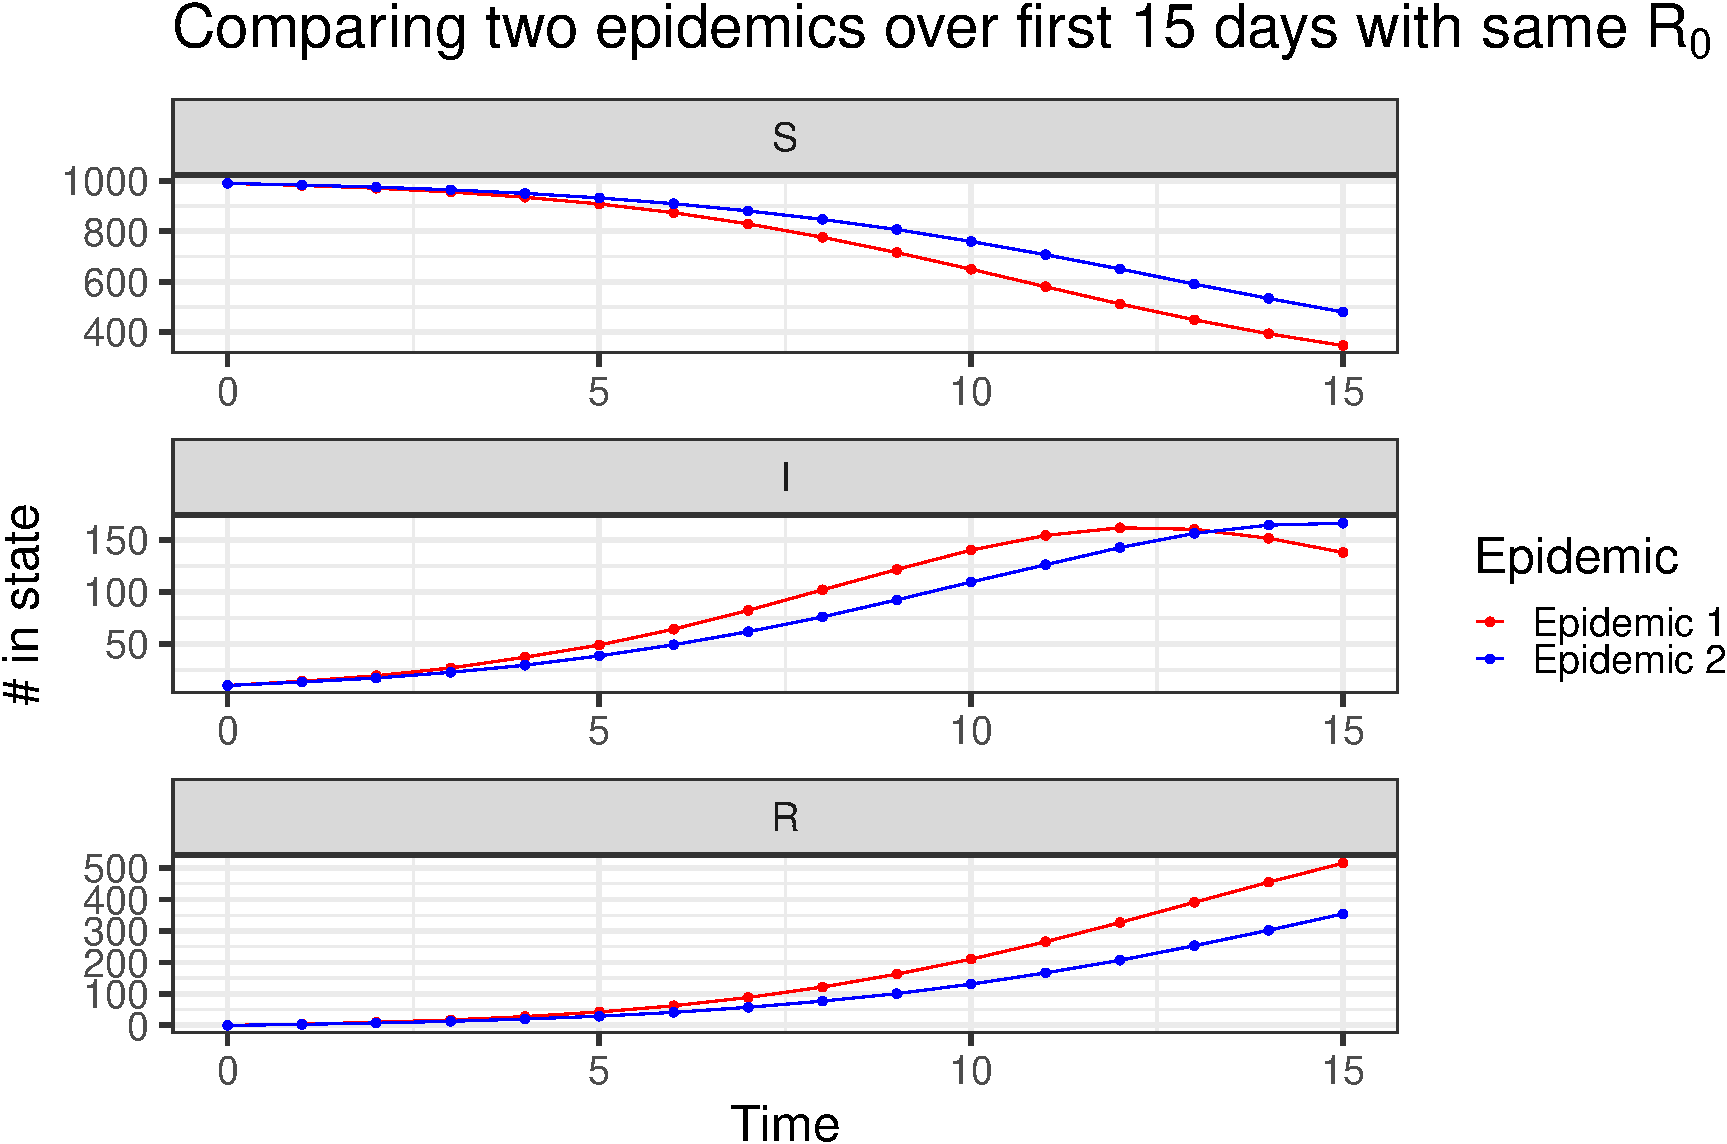
\includegraphics{Figs/unnamed-chunk-2-1} 

}

\caption{\label{fig:different-scales-standard}Example of two epidemics with different $\beta$ and $\gamma$ paremeters but the same initial reproduction number $R_0$ = 2.  Both plots are generated from models with $N= 1000$ individuals with $S(0) = 990$ and $I(0) = 10$.}\label{fig:unnamed-chunk-2}
\end{figure}
\end{CodeChunk}

\begin{CodeChunk}
\begin{figure}[H]

{\centering 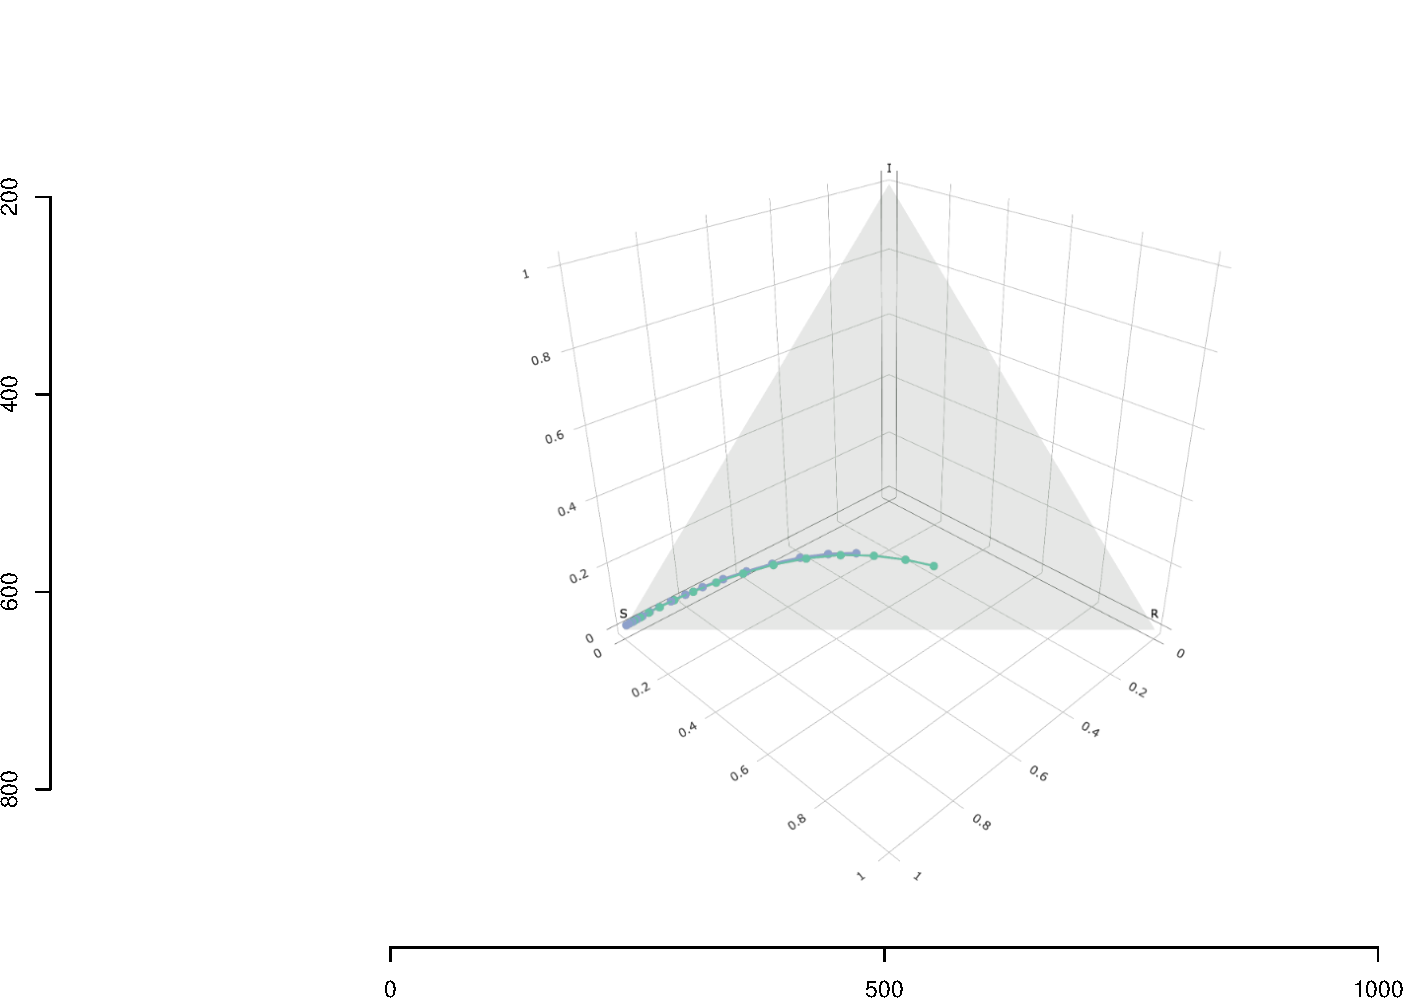
\includegraphics{Figs/unnamed-chunk-3-1} 

}

\caption{\label{fig:different-scales-tern}Example of two epidemics with different $\beta$ and $\gamma$ paremeters but the same initial reproduction number $R_0$ = 2.  Both plots are generated from models with $N= 1000$ individuals with $S(0) = 990$ and $I(0) = 10$.  These are plotted in the time-invariant view, where we can see the number of susceptible, infectious, and recovered.}\label{fig:unnamed-chunk-3}
\end{figure}
\end{CodeChunk}

\subsection[Beyond R0 and SIR]{\textcolor{violet}{Time-invariant analysis}
Beyond \(R_0\) and Kermack's and McKendrick SIR
Models}\label{beyond-r0-sir}

Through \textcolor{violet}{the} \(R_0\) \textcolor{orange}{example}, we
see that treating epidemics \textcolor{violet}{\sout{more}} like a
\sout{function of the time points in some higher dimensional space (nicely visualizable with a ternary plot for the SIR models)}
\textcolor{orange}{filaments embedded in a lower dimensional space}\textcolor{violet}{\sout{, then we can} allows us to}
better compare the overall structure of the epidemic and
\sout{how it impacted the population}
\textcolor{orange}{see how the population was directly impacted}.
\sout{Without knowing the generative structure underlying these two epidemics},
\textcolor{orange}{When the underlying generative model is unknown for epidemic trajectories},
we propose that time-invariant tools can help compare them in smart
ways, and that these ideas can extend past the CITE kermack1927 model
and to epidemics with more states.

\textcolor{violet}{
to be continued - (1) highlight filamental view of the epidemics through their simplex space (2) describe distances that could compare different epidemics with this mindset. Also motivate uncertainty for epidemics now that we have a filamental view (3) emphasis that this idea should extend to higher dimensions (4) present the idea that one could also compare bands together.
}

\section[Package overview]{Overview of
\pkg{EpiCompare}}\label{sec:overview}

\afterpage{\clearpage}
\begin{sidewaysfigure}[!ht]
    \centering
    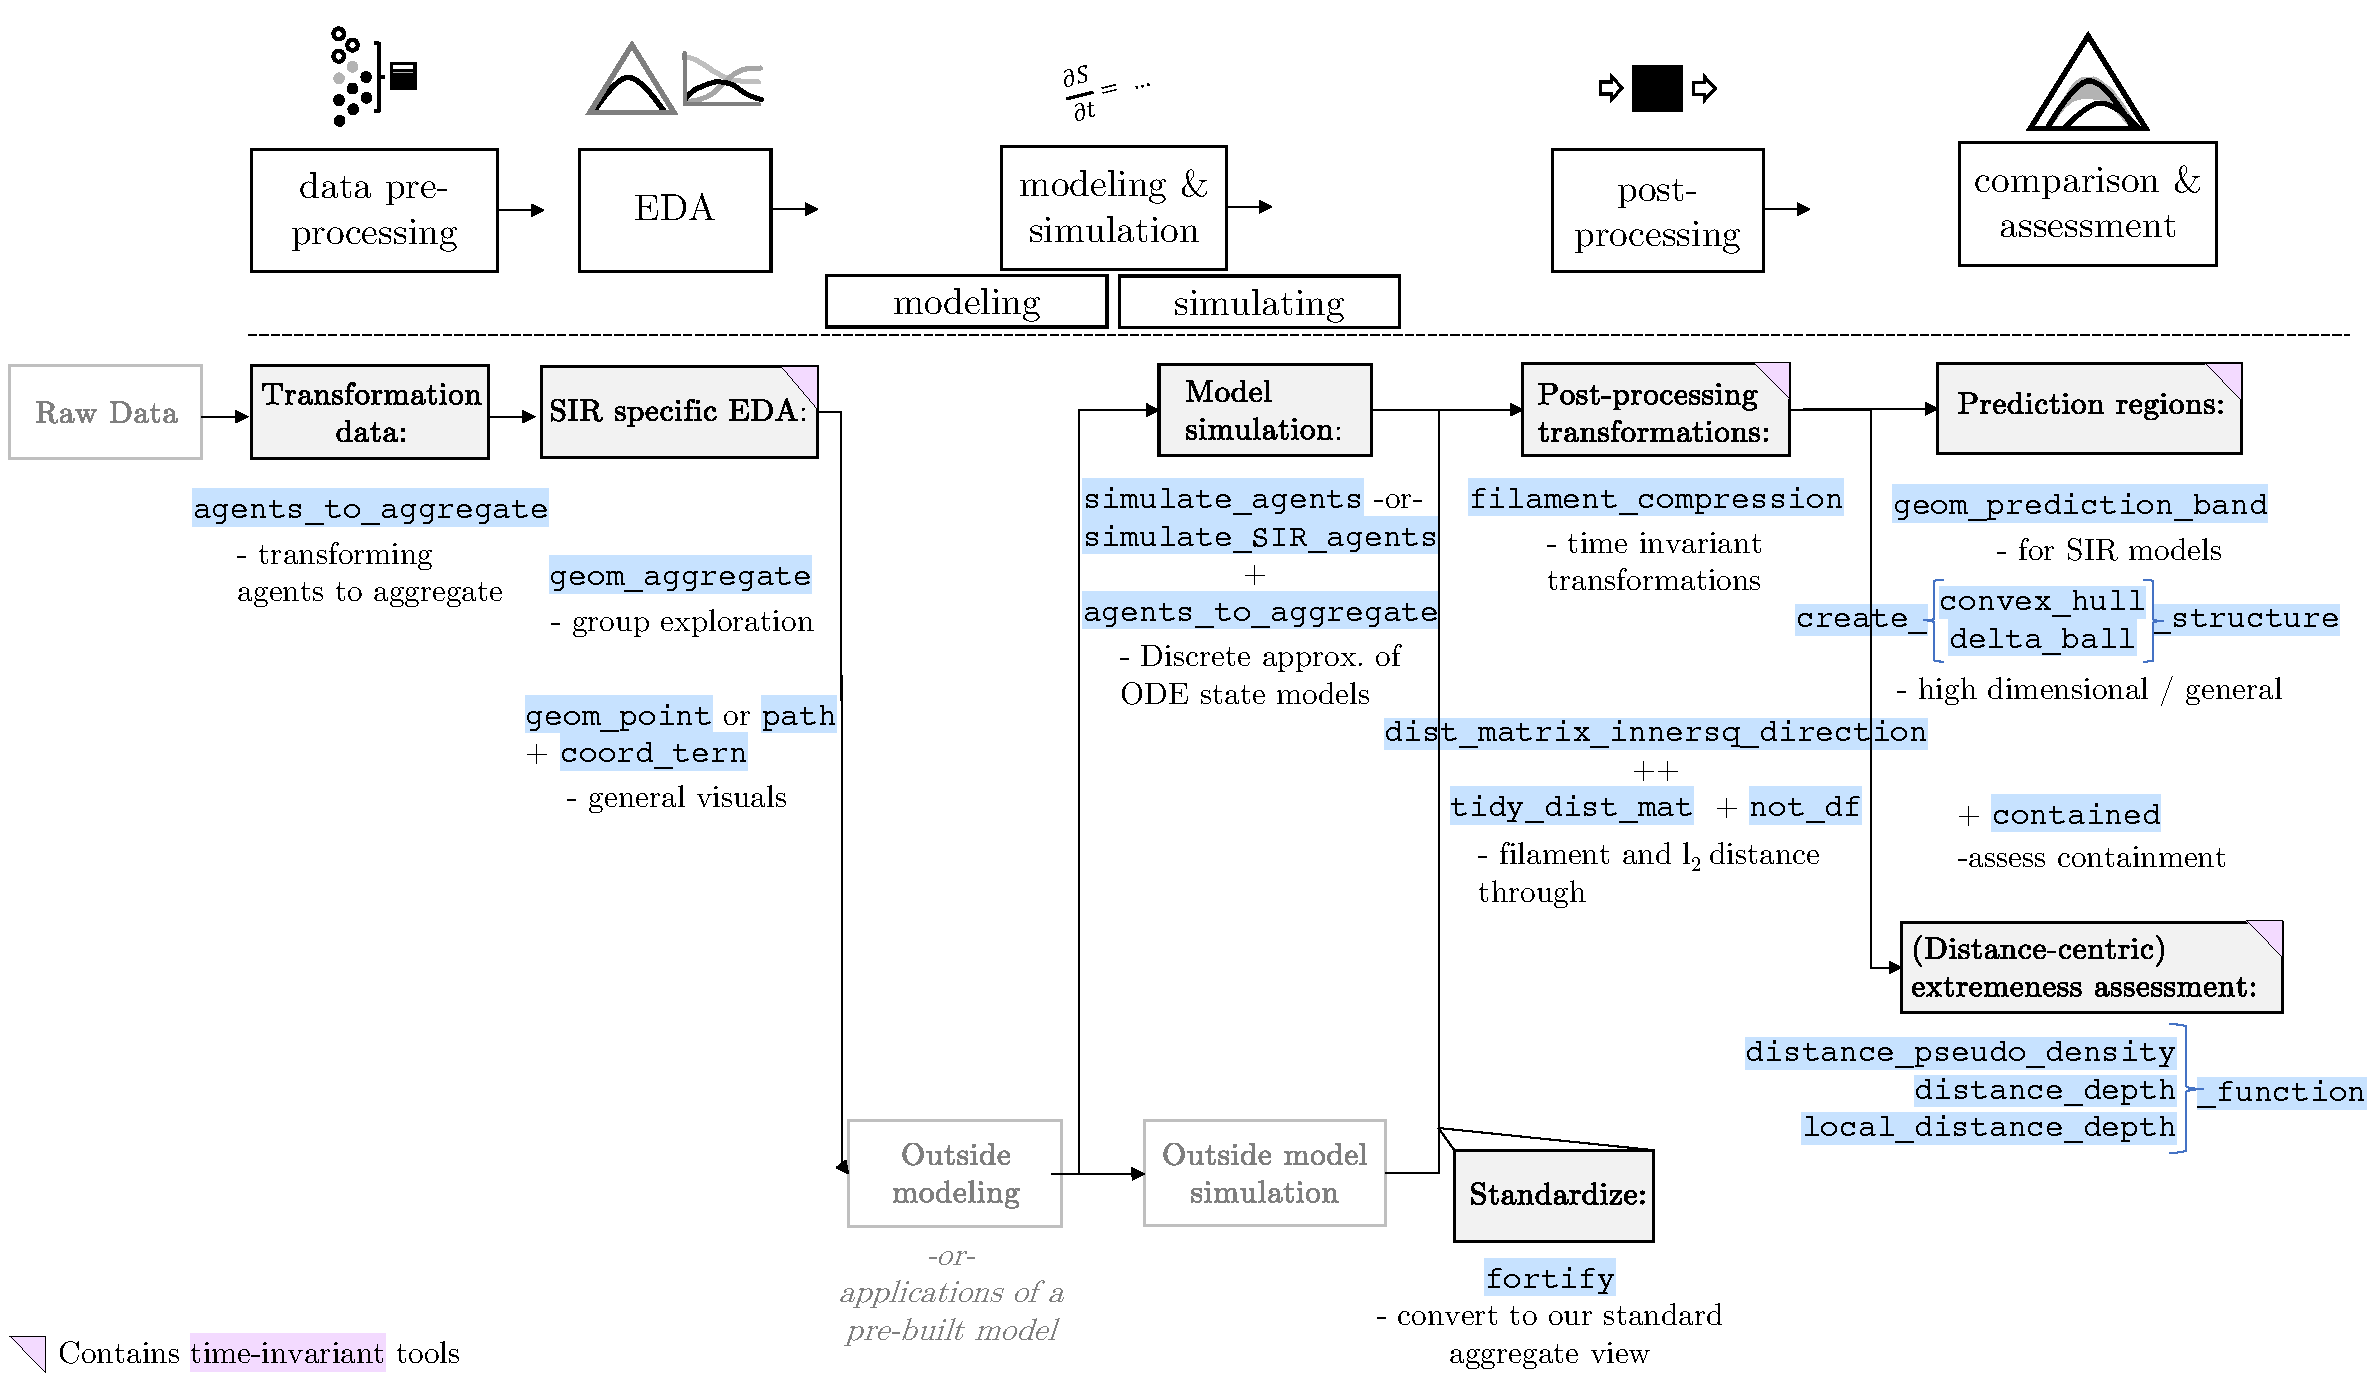
\includegraphics[width = 1\textwidth]{images/pipeline2_1.pdf}
    \caption{How \pkg{EpiCompare} supplements and aids in the epidemiological data analysis pipeline.}
    \label{fig:pipeline2}
\end{sidewaysfigure}

In this section, we present the tools implemented in \pkg{EpiCompare}
and explain how they aid in the data analysis pipeline. In Fig.
\ref{fig:pipeline2}, we illustrate how our package's functions fit into
the data analysis pipeline introduced in Fig. \ref{fig:pipeline}. All
front-facing functions are aimed to be as user-friendly as possible. We
also focus on providing the user ``tidyverse'' style functions, that
encourage piping and also follow clear verb naming schemes
\citep{Wickham2019}. Although users can typically incorporate
\pkg{EpiCompare} into any step in the data analysis process, there are
two primary points of entry. The first point of entry is the very
beginning with pre-processing and visualizing raw data, and the second
point of entry is after modeling and simulation. Figure
\ref{fig:pipeline2} captures these different paths, and we will
highlight\footnote{\textcolor{violet}{[Ben says: we need to make sure we actually do highlight ]}}
both approaches and how to leverage \pkg{EpiCompare} in the subsections
below.

\textbf{Data Pre-processing}

The first step of most data analysis is cleaning the data so it can be
explored. There are multiple ways to collect epidemiological data.
Sometimes individual records are collected, with times of different
states of the epidemic (infection, recovery, etc.) as well as individual
information like network structure, location, and sub-population
information. Other data collections focus on aggregate counts of
individuals in each epidemic state. In fact, usually only the number of
new infections at each time step (e.g.~weekly case counts) is observed.
Compartment totals (amounts of individuals in each state) are then
imputed from those case counts along with other information about the
disease and the population of interest. In \pkg{EpiCompare}, we focus on
understanding the overall impact of an outbreak at the
aggregate/population level, which allows for examination of overall
trends of an epidemic more easily.

In order to help the practitioner examine epidemics from an aggregate/
population lens, we provide a function called
\texttt{agents\_to\_aggregate}. This function transforms data about
individual/agents' initial entry into each state (e.g.~start of
infection, start of recovery, etc.) to an aggregate view of how many
individuals were in a state at a given time. There are often situations
where grouping agents into subpopulations (e.g.~subpopulations defined
by age or sex) can highlight different aggregate level trends. For
example, research by \citet{rvachev1985,anderson1992,worby2015} develop
state-based models that account for subpopulations. In \pkg{EpiCompare},
we facilitate subpopulation analysis by combining
\pkg{dplyr}::\texttt{group\_by} and \texttt{agent\_to\_aggregate} to
provide aggregation at a group level.

The \texttt{agents\_to\_aggregate} function is flexible and can deal
with a wide range of information about each individual. It can,
theoretically, account for infinitely many states. This functionality
allows the practitioner to aggregate information relative to the
standard states (e.g.~``Susceptible'', ``Infectious'', and
``Recovered'') as well as add states (e.g.~``Exposed'', ``iMmune'',
``Hospitalized'')
(CITE\footnote{\textcolor{violet}{[Ben says: this was originally to back up the claim that SIR is the "standard" states - now we might need to have a paper that says that SIR is the standard states and also suggests other states...]}}).
Additionally, \texttt{agents\_to\_aggregate} also permits indicators for
death/exit and birth/entry dates. Overall, the function
\texttt{agents\_to\_aggregate()} is a powerful tool for pre-processing
data.

\textbf{EDA}

With raw data, ``getting to know'' our data currently means figuring out
good combinations of visualizations, numerical summaries and subsets. An
expert coder has many ways to successfully explore the data in an
aggregate lens using \texttt{agents\_to\_aggregate}. \pkg{EpiCompare}
also includes tools to rapidly explore data that has three epidemic
states. Building on the tools in \pkg{ggplot2} and \pkg{ggtern}, our
\texttt{geom\_aggregate} provides a rapid way to explore different
subpopulations' experience of an epidemic by combining the ideas behind
\texttt{agents\_to\_aggregate} for three-state models to examine
subpopulation trajectories in a 3d simplex space
\citep{Wickham2016, Hamilton2018}.
\textcolor{orange}{[Shannon says: come back?]}\footnote{\textcolor{violet}{[Ben says: what does this note mean?]}}
Visualization tools for three-state models were developed because (1)
SIR models are some of the most common and basic epidemic state-based
models and (2) our simplex representation of these epidemics emphasizes
a ``time-invarance'' representation of the data (for a refresher see
Section \ref{sec:time-invariant}).
\textcolor{orange}{[Shannon says: make sure SIR is defined before.]}

\textbf{Model Fitting and Simulations}

\textcolor{violet}{[Ben says: think about this section and if it highlights that we can bring in outside models...]}

\textcolor{violet}{After getting a good sense of what a past or current epidemice looks like through EDA, the next step is often model fitting and/or simulations. In this step, and the next step (post-processing), we discuss how to include practioners' use of tools to create models and simulations that exist outside of \pkg{EpiCompare}.}
This package does not focus on fitting a model to data, we do provide
some flexible functions for simulation of basic discrete-time
epidemic-state models.
\textcolor{violet}{After estimating or predicting transition rates between states,}
these functions produce individual level
\textcolor{violet}{simulations\sout{information}} and can be
\textcolor{violet}{\sout{naturally}} combined with
\texttt{agents\_to\_aggregate()} to view these simulations through an
aggregate lens. The function \texttt{simulate\_SIR\_agents()} simulates
an SIR epidemic with user inputs for the number of simulations, the
initial number in each state, the infection and recovery parameters
\((\beta, \gamma\)), and the total number of discrete time steps. This
function allows for easy access to SIR model analysis and comparison.
Beyond SIR models, the function \texttt{simulate\_agents()} takes as
input a user-specified transition matrix and other epidemic parameters
to allow the user to create simulations of an outbreak for \textit{any}
number of states and any number of transitions among them. This
flexibility in states can be used to also reflect group-based dynamics.
This allows for users to explore the space of models in an intuitive way
without getting bogged down by too much mathematical detail. For
consistency, we have made output from \texttt{simulate\_agents()} and
\texttt{simulate\_SIR\_agents()} compatible with
\texttt{agents\_to\_aggregate()} so aggregate information may easily be
accessed.

\textbf{Post-processing}

\textcolor{violet}{[Ben says: I think we should remind the reader that we care more about simulations, in order to compare fitted models between themselves and the true epidemics.]}

\textcolor{violet}{[Ben says: this replaces the first paragraph below]}

\textcolor{violet}{If the practitioner wishes to compare between models and with their true epidemics, one needs to process their models and simulations.}
\textcolor{violet}{In general, [p}ost-processing of modeling and
simulation consists of making summary statistics, plots, tables, and
other ways to disseminate information to the public.{]}
\textcolor{violet}{The summaries can be very complex, and a}{[}s a
result, a number of epidemic modeling \textcolor{violet}{\proglang{R}}
packages return a special class, specific to their modeling. The special
classes often contain a plethora of information from residuals, model
diagnostics, input parameters, and more. While incredibly useful, these
special classes can be difficult for novice coders to navigate.{]}

\textcolor{violet}{[Ben says: replaced with above paragraph]}
Post-processing of modeling and simulation consists of making summary
statistics, plots, tables, and other ways to disseminate information to
the public. For example, comma separated value files (\texttt{.csv}) are
a standard way to share information within tables. However, model output
is often far more complicated than what a traditional \texttt{.csv}
would allow. \textcolor{orange}{Do we need three sentences about csvs?}
As a result, a number of epidemic modeling packages return a special
class, specific to their modeling. The special classes often contain a
plethora of information from residuals, model diagnostics, input
parameters, and more. While incredibly useful, these special classes can
be difficult for novice coders to navigate.

To this end, we have \textcolor{violet}{provide\sout{adapted}} a series
of \texttt{fortify}-style
\textcolor{violet}{methods\sout{functions}}\footnote{\textcolor{violet}{[Ben says: Not tied to this change.]}},
called \texttt{fortify\_aggregate()} which transform output from
packages like \pkg{pomp} and \pkg{EpiModel} into tidy-styled data frames
which contain information about the total number of individuals in each
state at a given time, for a given simulation. These fortify functions
have output that is consistent with that of
\texttt{agents\_to\_aggregate()}.

\textcolor{violet}{[Ben says: new paragraph]} To utilize simulations
epidemics in later time-invariant analysis we also provide a function to
convert temporally defined epidemics to filamental representations.
Specifically, we provide the function \texttt{filament\_compression} to
convert simulation(s) to filaments as expressed by presenting the
epidemic as a ordering of some common fixed number of points so that
they are equally spaced along the original path in the proportional
state
space\footnote{\textcolor{violet}{[Ben: this should be cleaned up.]}}.

\textbf{Comparisons and Assessment}

\textcolor{violet}{[This still needs to be worked on - just a reminder.]}

Comparison and assessment of model fit or comparisons of one model to
another model can be performed in a variety of ways including mean
square error, AIC, plots, and more. Perhaps the most useful tool
\pkg{EpiCompare} has to offer to the expert, for comparison and
assessment of models, is in its post-processing tools which create a
standard output. It is then a matter of writing a script or function
made for that standard output to assess the results from multiple models
in the way the user desires.

However, for those who like more concrete tools, \pkg{EpiCompare} offers
functions to compare prediction regions to one another including
\texttt{geom\_prediction\_band()} (which plots the region), and
\texttt{create\_\{convex\_hull,delta\_ball\}\_structure()}(which returns
the \texttt{R} output for the given structure), and \texttt{contained()}
(which allows the user to determine if one set of points is contained in
a prediction band). Additionally, we offer ways to determine if model
outputs are compatible with one another, that is how extreme one output
is to another. \textcolor{orange}{Ben says something about distance}

\section[Tour]{A tour of \pkg{EpiCompare}}\label{sec:tour}

In this section, we highlight a number of the functionality available in
\pkg{EpiCompare}. These functionality include data cleaning,
visualization, simulation, and comparison, in accordance with the data
analysis pipeline \ref{fig:pipeline}. We show a full data analysis from
beginning to end that can be accomplished in a streamlined and
standardized manner.

\subsection{Data and exploratory analysis}

We analyze an outbreak of measles in the town of Hagelloch, Germany from
1861-1862, a data set organized by \cite{pfeilsticker1863}. The data was
later made visible by \cite{oesterle1992} and made available in an
\proglang{R} by \cite{surveillance2017}. The Hagelloch data includes a
rich set of features including household members, school level,
household locations, date of first symptoms (prodromes), date of measles
rash, and even the alleged infector. A subset of the data is shown in
Table \ref{tab:hags-people}. Because of these rich features, this data
set has been an ideal testing ground methodology in infectious disease
epidemiology and is used in work by
\cite{Neal2004,britton2011,groendyke2012,becker2016}.

\begin{CodeChunk}
\begin{table}[!h]

\caption{\label{tab:hags-people}Subset of Hagelloch infection data.  Features include the person ID, household ID (HH ID), age, sex, class level (Pre-K/1st/2nd), date of first symptoms, date of the appearance of the measles rash, and the alleged infector ID of the individual.}
\centering
\begin{tabular}[t]{rrlrllllr}
\toprule
ID & HH ID & Name & Age & Sex & Class & Symp. Start & Rash Date & Infector ID\\
\midrule
1 & 61 & Mueller & 7 & female & 1st class & 1861-11-21 & 1861-11-25 & 45\\
2 & 61 & Mueller & 6 & female & 1st class & 1861-11-23 & 1861-11-27 & 45\\
3 & 61 & Mueller & 4 & female & preschool & 1861-11-28 & 1861-12-02 & 172\\
4 & 62 & Seibold & 13 & male & 2nd class & 1861-11-27 & 1861-11-28 & 180\\
5 & 63 & Motzer & 8 & female & 1st class & 1861-11-22 & 1861-11-27 & 45\\
45 & 51 & Goehring & 7 & male & 1st class & 1861-11-11 & 1861-11-13 & 184\\
\bottomrule
\end{tabular}
\end{table}

\end{CodeChunk}

With \pkg{EpiCompare}, we can easily obtain the empirical cumulative
incidence function with respect to the measles rash appearance (variable
\code{ERU}) with the following tidy-style function,
\code{agents_to_aggregate}. The function \code{agents_to_aggregate} is a
key component of \pkg{EpiCompare}, allowing the user to easily switch
from an individual-level (i.e.~an agent) view of a disease to an
aggregate level. For example, the below code shows how we can convert
the agent data to a cumulative incidence of the measles rash, in order
to see how the disease spread through the population over time. We can
then compare the cumulative incidence of the rash to the cumulative
incidence of the prodromes, i.e.~the initial symptoms. We do this with
the below code, and a part of the cumulative incidence data output are
shown in Table \ref{tab:cif-rash}. The argument
\code{integer_time_expansion} indicates whether we should include all
time points in the recorded range of the data or only when there is a
change in the incidence.

\begin{CodeChunk}
\begin{CodeInput}
R> cif_rash  <- hagelloch_raw %>%
+   mutate(time_of_rash = as.numeric(ERU - min(PRO, na.rm = TRUE))) %>%
+   agents_to_aggregate(states = time_of_rash,
+                       integer_time_expansion = FALSE) %>%
+   mutate(type = "Rash")
\end{CodeInput}
\end{CodeChunk}

\begin{CodeChunk}
\begin{table}[!h]

\caption{\label{tab:cif-rash}Turning the individual-level information from the Hagelloch data to an aggregate view of the cumulative incidence of the measles rash in the population over time.}
\centering
\begin{tabular}[t]{rrr}
\toprule
Time & \# Susceptible & \# Total rash appearances\\
\midrule
0 & 188 & 0\\
4 & 187 & 1\\
7 & 186 & 2\\
9 & 185 & 3\\
12 & 183 & 5\\
\bottomrule
\end{tabular}
\end{table}

\end{CodeChunk}

One question of interest is the duration between initial onset of
prodromes or symptoms and the appearance of the measles rash. Since
\code{agent_to_aggregate} outputs a tidy-style data frame, it is a
simple task to plot the two sets of incidence curves on the same graph
(Fig. \ref{fig:cifs}).

\begin{CodeChunk}
\begin{CodeInput}
R> cif_prodromes <- hagelloch_raw %>%
+   mutate(time_of_PRO = as.numeric(PRO - min(PRO, na.rm = TRUE))) %>%
+   agents_to_aggregate(states = time_of_PRO,
+                       integer_time_expansion = FALSE) %>%
+   mutate(type = "Pro")
\end{CodeInput}
\end{CodeChunk}

\begin{CodeChunk}
\begin{CodeInput}
R> plot_df <- bind_rows(cif_rash, cif_prodromes)
R> 
R> ggplot(data = plot_df,
+        aes(x = t, y = X1, col = type)) + 
+   geom_step() + 
+   labs(title = "Cumulative incidence of measles appearance",
+        x = "Time (days relative to first prodrome appearance)",
+        y = "Cumulative incidence of event") + 
+   coord_cartesian(xlim = c(0, 55)) +
+   scale_color_manual(values = c("blue", "red"))
\end{CodeInput}
\begin{figure}[H]

{\centering 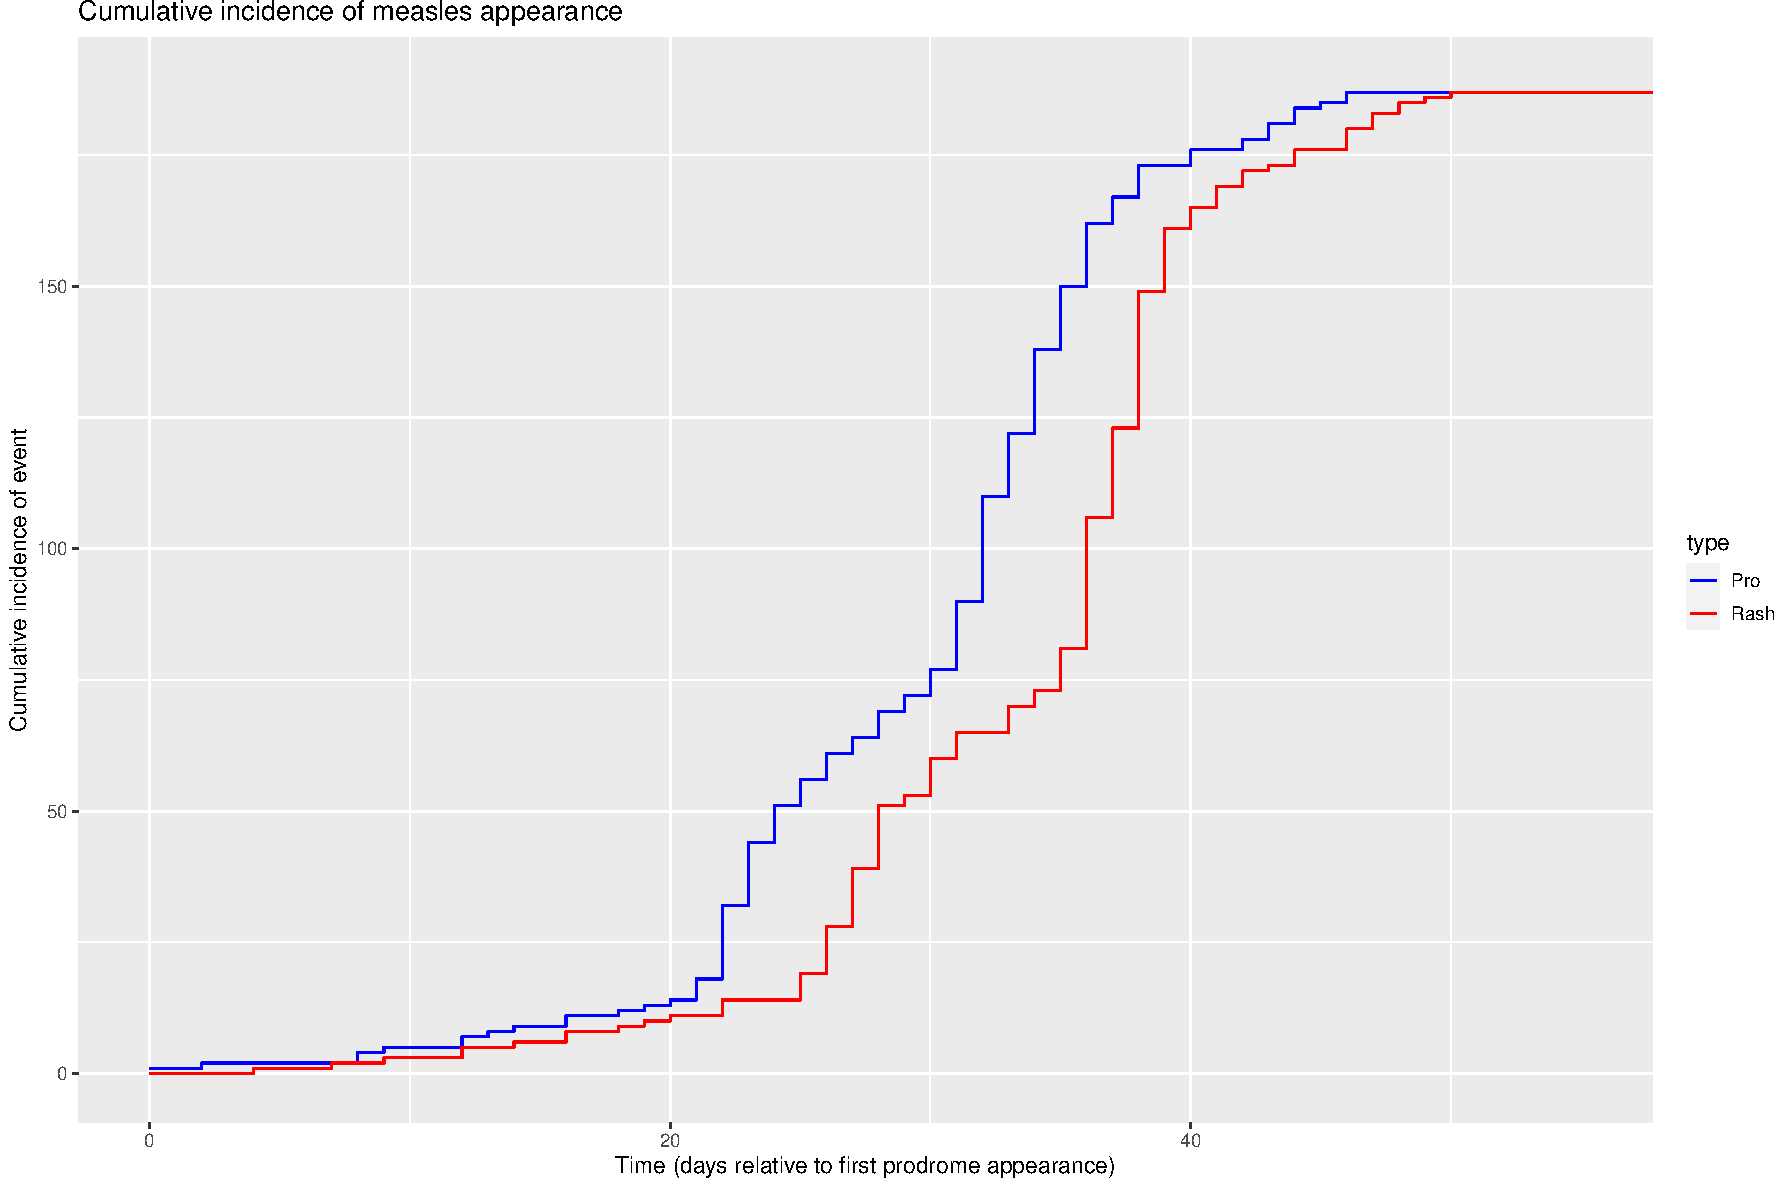
\includegraphics{Figs/unnamed-chunk-7-1} 

}

\caption{\label{fig:cifs}Empirical cumulative incidence functions of prodrome (symptom) onset and measles rash appearance.  We see that there is approximately a a constant lag between the two curves.}\label{fig:unnamed-chunk-7}
\end{figure}
\end{CodeChunk}

The real power of \code{agents_to_aggregate()} lies in its ability to
aggregate over any number of pre-specified states. For example, the
Hagelloch data sets contains two columns, \code{tI} and \code{tR}, the
time of infection and recovery, respectively of each individual. We can
then plot the SIR values through a time-invariant lens using
\pkg{ggplot2} and \pkg{ggtern} functions (as shown in Fig.
\ref{fig:hag-tern-raw}) or with our custom \code{geom},
\code{geom_aggregate}, which takes the raw agent data as input.

\begin{CodeChunk}
\begin{CodeInput}
R> hagelloch_sir <- hagelloch_raw %>%
+   agents_to_aggregate(states = c(tI, tR),
+                       min_max_time = c(0, 55)) %>%
+   rename(time = t, S = X0, I = X1, R = X2)
R> 
R> 
R> ggplot(hagelloch_sir, aes(x = S, y = I, z = R))+
+   coord_tern() +
+   geom_path() +
+   labs(x = "S", y = "I", z = "R",
+        title = "Time invariant view of Hagelloch measles outbreak") + 
+   theme_sir(base_size = 24)
\end{CodeInput}
\begin{figure}[H]

{\centering 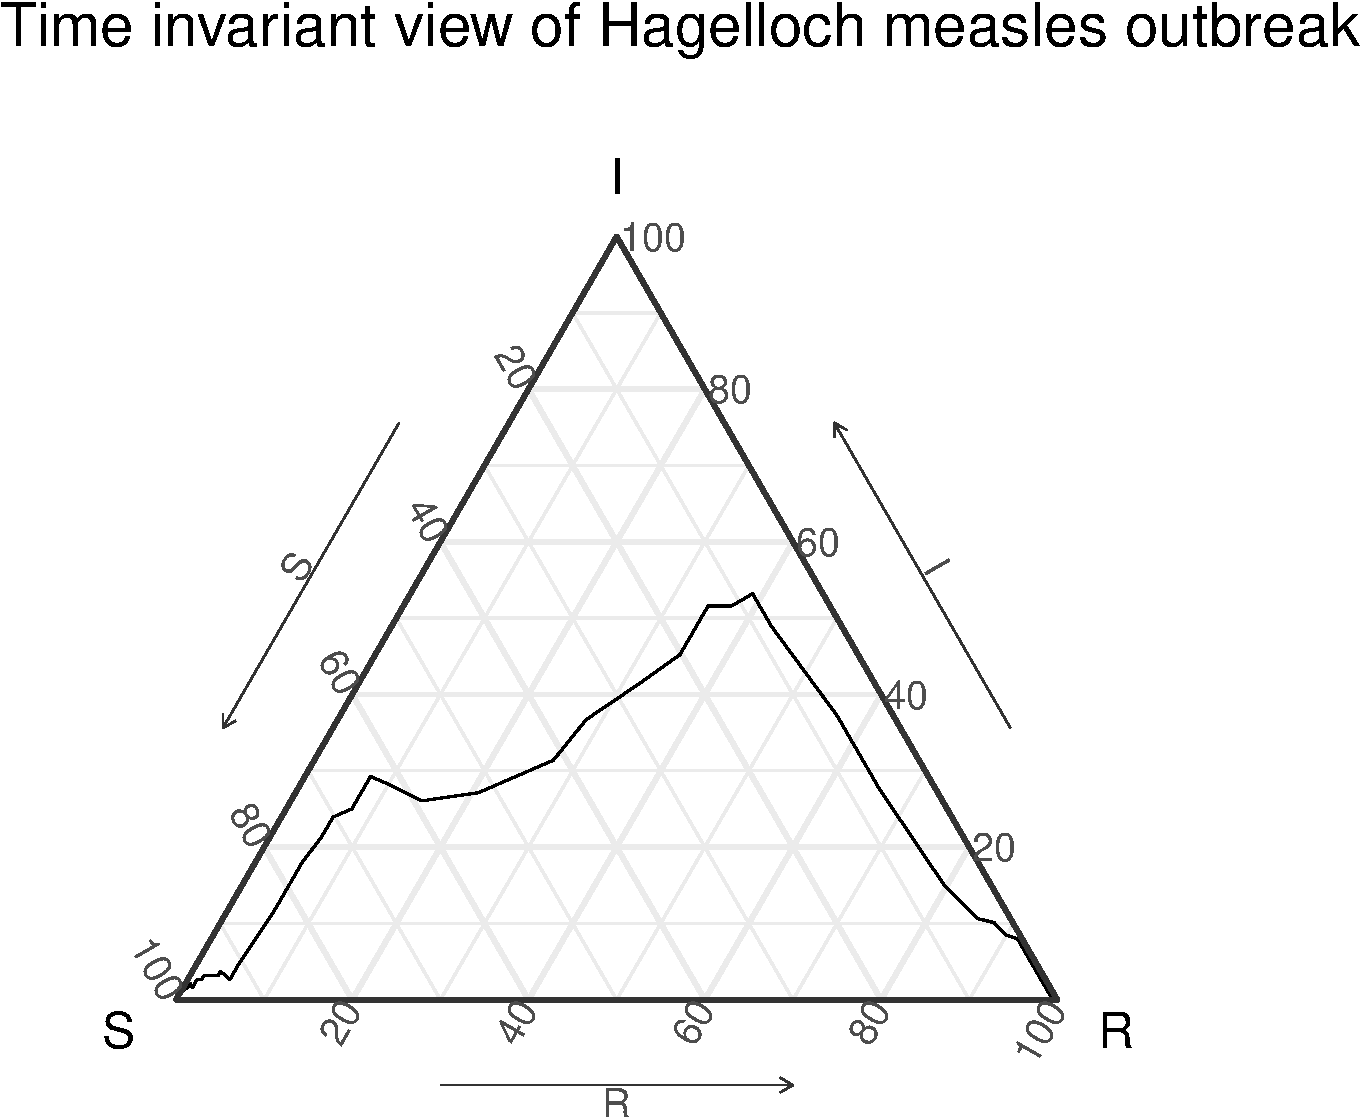
\includegraphics{Figs/unnamed-chunk-9-1} 

}

\caption{\label{fig:hag-tern-raw}Time invariant view of the Hagelloch epidemic where we view the individuals in Susceptible, Infectious, or Recovered states.  We see there are two peaks of infection (the vertical axis).}\label{fig:unnamed-chunk-9}
\end{figure}
\end{CodeChunk}

Moreover, we can look at the outbreaks of the disease by group within
\code{agent_to_aggregate()} or \code{geom_aggregate()}. This allows us
to examine differences among the different groups of individuals. For
example, we show the time invariant outbreak by class level in Figure
\ref{fig:tern-class-data}. Immediately, we see that time invariant
infection curve is different for the pre-school class compared to the
1st class. In the 1st class, we see about 95\% of the class become
infected and less than 10\% of them having recovered, which is
indicative of a super-spreading event. This suspicion is further
confirmed in that 26 of the 30 1st class students have been reportedly
infected by the same individual.

\begin{CodeChunk}
\begin{CodeInput}
R> hagelloch_raw %>%
+   ggplot(aes(y = tI, z = tR, color = CL)) +
+   geom_aggregate(size = 2) + coord_tern() +
+   labs(x = "S", y = "I", z = "R",
+        color = "Class") +
+   scale_color_brewer(palette = "Dark2") +
+   facet_wrap(~CL)
\end{CodeInput}
\begin{figure}[H]

{\centering 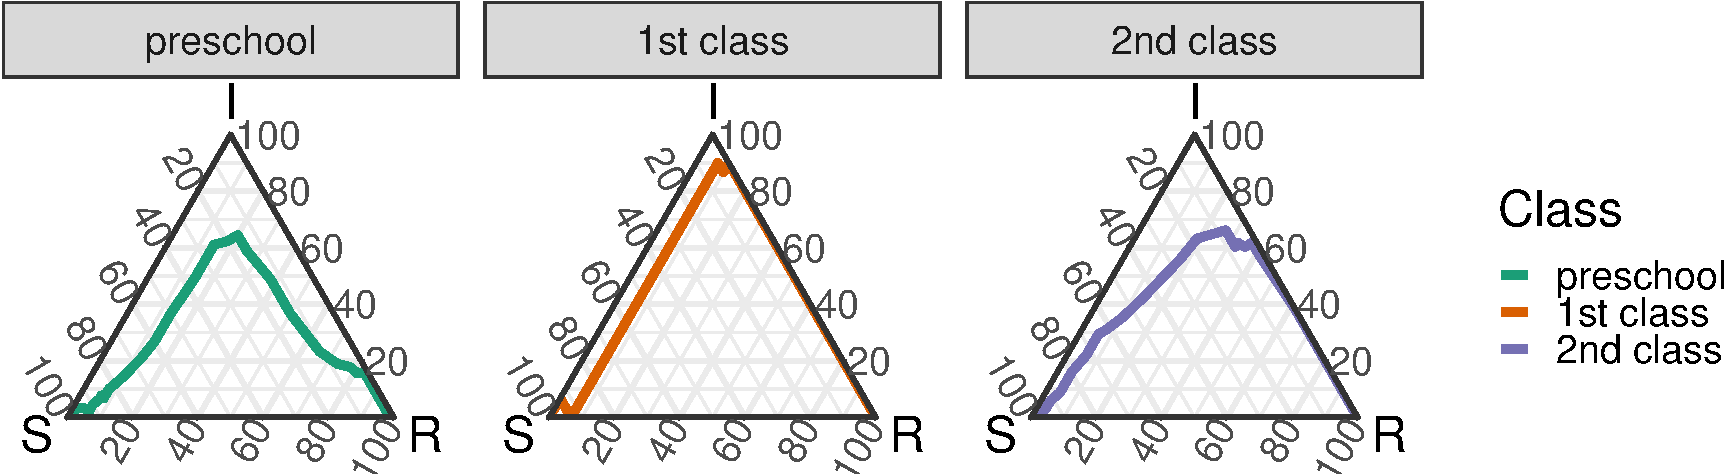
\includegraphics{Figs/unnamed-chunk-10-1} 

}

\caption{\label{fig:tern-class-data}Time invariant outbreak curves for the three class groups.  The pre-school class has a distinct peak of infection whereas the peak infection point for the other two classes are less well defined.}\label{fig:unnamed-chunk-10}
\end{figure}
\end{CodeChunk}

Along with multiple epidemic states, the function
\code{agents_to_aggregate} can also be extended to populations with
vital dynamics (e.g.~birth and death) and examples of this are shown in
the package vignette. In summary, \code{agents_to_aggregate()} is a
multi-purpose workhorse that may be leveraged to convert individual
level records into aggregate information that may be more useful for
some forms of epidemic modeling such as compartment modeling.

Up to this point, we have used \pkg{EpiCompare} in the context of
observed data. We also want to compare statistical models, and
\pkg{EpiCompare} aids in that process via a simple but dynamic
individual-level data generator, conversion tools for popular epidemic
model packages, and model assessments. We demonstrate an example here.

We first try to model the Hagelloch data with a stochastic SIR model,
which we refer to as the `simple SIR.' In our vignette, we show how to
fit this simple SIR model via maximum likelihood and simulate from the
model with those best fit parameters. Our function
\code{simulate_agents()} generates individual level data according to
discrete time multinomial draws, which depend on the number of
individuals in each state at the previous time step and a matrix of
transition probabilities. For example, the below code generates 100
simulations of an outbreak of a disease with one initial infector in a
population of \(n= 188\) individuals.

\begin{CodeChunk}
\begin{CodeInput}
R> trans_mat <- matrix(c("X0 * (1 - X1 * par1 / N)", "X0 * X1  * par1 / N", "0",
+                   "0", "X1 * (1 - par2)", "par2 * X1",
+                   "0", "0", "X2"), byrow = TRUE, nrow = 3)
\end{CodeInput}
\end{CodeChunk}

\begin{CodeChunk}
\begin{CodeInput}
R> set.seed(2020)
R> 
R> best_params <- c("beta" = .36, "gamma" = .13)
R> ## This is the SIR representation
R> 
R> rownames(trans_mat) <- c("S", "I", "R")
R> init_vals <- c(187, 1, 0)
R> par_vals <- c(par1 = best_params[1], par2 = best_params[2])
R> max_T <- 55
R> n_sims <- 100
R> 
R> agents <- simulate_agents(trans_mat,
+                        init_vals,
+                        par_vals,
+                        max_T,
+                        n_sims,
+                        verbose = FALSE)
\end{CodeInput}
\end{CodeChunk}

\begin{CodeChunk}
\begin{CodeInput}
R> agg_model <- agents %>% group_by(sim) %>%
+   agents_to_aggregate(states = c(I, R)) %>%
+   mutate(Type = "Simple SIR")
\end{CodeInput}
\end{CodeChunk}

The result of our simulation is the object \code{agents} which is a
18800 \(\times\) 5 data frame, which details the time of entry into the
\(S\), \(I\), and \(R\) states for a given simulation. Before we examine
the results of this simple SIR model, we will also examine another, more
sophisticated SIR model, this time from the package \pkg{EpiModel}.
Briefly, this model first fits a contact network to the set of
indivduals, where the class of the student is a covariate. The model
then simulates a SIR-epidemic on that network.

\begin{CodeChunk}
\begin{CodeInput}
R> library(EpiModel)
R> ## WARNING:  Will take a minute or two
R> 
R> set.seed(42)
R> nw <- network.initialize(n = 188, directed = FALSE)
R> nw <- set.vertex.attribute(nw, "group", rep(0:2, each = 90, 30, 68))
R> formation <- ~edges + nodematch("group") + concurrent
R> target.stats <- c(200, 300, 200)
R> coef.diss <- dissolution_coefs(dissolution = ~offset(edges),  duration = 5)
R> est1 <- netest(nw, formation, target.stats, coef.diss, edapprox = TRUE)
R> 
R> param <- param.net(inf.prob = 0.1, act.rate = 5, rec.rate = 0.1)
R> status.vector <- c(rep(0, 90), rep(0, 30), rep(0, 67), 1)
R> status.vector <- ifelse(status.vector == 1, "i", "s")
R> init <- init.net(status.vector = status.vector)
R> control <- control.net(type = "SIR", nsteps = 55,
+                        nsims = 100, epi.by = "group")
R> epimodel_sir <- netsim(est1, param, init, control)
\end{CodeInput}
\end{CodeChunk}

The output of this model is \code{epimodel_sir}, an object of class
\code{netsim}, which contains a plethora of modeling information. We
provide the function \code{fortify_aggregate()}, which can take objects
from specialized classes of modeling output and transform it into a
tidy-style data frame.

\begin{CodeChunk}
\begin{CodeInput}
R> fortified_net <- fortify_aggregate(epimodel_sir, 
+                                    states = c("s.num", "i.num", "r.num")) %>%
+   mutate(Type = "EpiModel SIR",
+          sim = as.numeric(gsub("sim", "", sim)))
\end{CodeInput}
\end{CodeChunk}

We can then analyze the results of the two models side by side as
time-invariant epidemic curves. The results are shown in Figure
\ref{fig:hag-simple-sir}, where a 90\% prediction band is estimated from
the delta ball method for each of the two models. For the Simple SIR
model, we see that the data generally covers the data fairly well but
clearly misses the second peak of infection. We also see that the
prediction band is very large, covering up a large area of the ternary
plot. On the other hand, for the \pkg{EpiModel} model, we see that the
prediction band covers the data quite well and takes up less area.

\begin{CodeChunk}
\begin{CodeInput}
R> both_models <- bind_rows(agg_model, fortified_net)
R> 
R> 
R> g <- ggplot() + geom_prediction_band(data = both_models %>% filter(t != 0),
+          aes(x = X0, y = X1, z = X2,
+               sim_group = sim, fill = Type),
+          alpha = .5,
+          conf_level = .90) 
\end{CodeInput}
\end{CodeChunk}

\begin{CodeChunk}
\begin{CodeInput}
R> g +   geom_path(data = both_models %>% filter(t !=0),
+             aes(x = X0, y = X1, z = X2, group = paste(Type, sim)),
+             alpha = .3, col = "gray40") + 
+     coord_tern() + theme_sir(base_size = 24) +
+   geom_point(data = hagelloch_sir,
+              aes(x = S, y = I, z =R), col = "black") +
+   labs(title = "Simple SIR model",
+        subtitle = "90% Prediction band and original data",
+        x = "S", y = "I", z = "R") +
+   scale_fill_manual(values = c("#006677", "#AA6600")) + 
+   facet_wrap(~Type) +
+   theme(legend.position = "bottom")
\end{CodeInput}
\begin{figure}[H]

{\centering 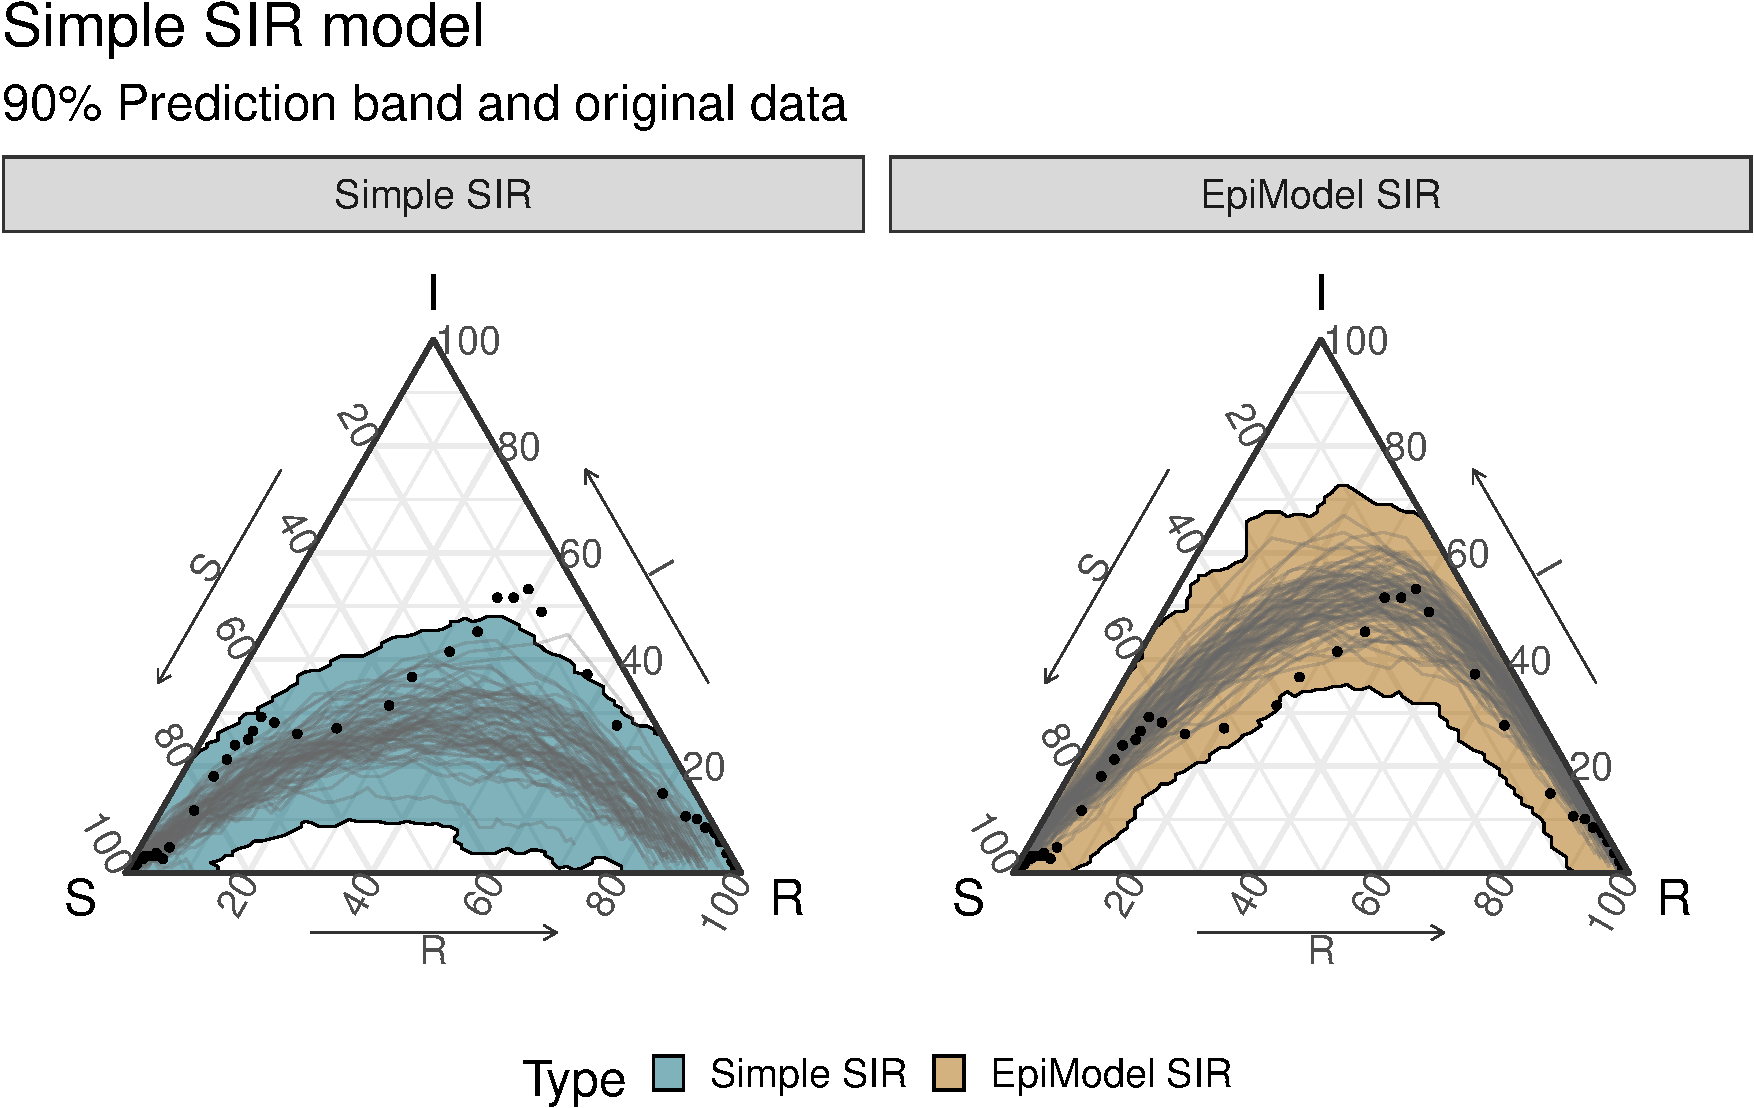
\includegraphics{Figs/unnamed-chunk-17-1} 

}

\caption{\label{fig:hag-simple-sir}  Original Hagelloch SIR data (black) along with 90\% prediction band and actual simulation paths from the Simple SIR and the EpiModel SIR models.}\label{fig:unnamed-chunk-17}
\end{figure}
\end{CodeChunk}

However, both models are not a good fit to the filamental path as
opposed to the individual points in \((S, I, R)\)-space. This can be
captures with the set of simulations both models predict, which all
generally have a single defined peak of infection whereas the data
certainly looks like it has two distinct peaks, likely caused by our
assumed super-spreader event. This observation is backed up by the below
analysis that demonstrates that the estimated psuedo-density of the
observed epidemic (relative to the simulations from either model) is
much less likely then \textbf{any} of the simulations (reported in Table
\ref{tab:hags-extreme}. In conclusion, \pkg{EpiCompare} makes it clear
that, at a glance, 1) the EpiModel network model is a better fit than
the Simple SIR model, and 2) the fit is only good at the individual
point level as opposed to the epidemic path level.

\begin{CodeChunk}
\begin{CodeInput}
R> #-- after cleaning up and combining --
R> all_together_df <- rbind(simple_sir,
+                          hagelloch_sir2)
\end{CodeInput}
\end{CodeChunk}

\begin{CodeChunk}
\begin{table}[!h]

\caption{\label{tab:cif-all-together-df}Top and bottom 2 rows of \tt{all\_together\_df}\text{, combining both simulated epidemics and the true epidemic.}}
\centering
\begin{tabular}[t]{lrrrrr}
\toprule
Type & sim & t & S & I & R\\
\midrule
Simple SIR & 1 & 0 & 188 & 0 & 0\\
Simple SIR & 1 & 1 & 187 & 1 & 0\\
true observation & 0 & 54 & 1 & 0 & 187\\
true observation & 0 & 55 & 1 & 0 & 187\\
\bottomrule
\end{tabular}
\end{table}

\end{CodeChunk}

\begin{CodeChunk}
\begin{CodeInput}
R> compression_df <- all_together_df %>% group_by(Type, sim) %>% 
+   filament_compression(data_columns = c("S","I","R"), 
+                        number_points = 20)
\end{CodeInput}
\end{CodeChunk}

\begin{CodeChunk}
\begin{CodeInput}
R> tdmat <- compression_df %>% 
+   dist_matrix_innersq_direction(
+     position = c(1:length(compression_df))[
+       names(compression_df) %in% c("S","I", "R")],
+     tdm_out = T)
R> 
R> simple_sir_true_obs_info <- tdmat %>% 
+   compare_new_to_rest_via_distance(
+     new_name_id = data.frame(Type = "true observation", sim = 0),
+     distance_func = distance_psuedo_density_function, 
+     sigma = "20%") 
\end{CodeInput}
\end{CodeChunk}

\begin{CodeChunk}
\begin{table}[!h]

\caption{\label{tab:hags-extreme}The extremeness of the true simulations based on comparing psuedo-density estimates between true vs simulated curves}
\centering
\begin{tabular}[t]{l>{\raggedleft\arraybackslash}p{6cm}>{\raggedleft\arraybackslash}p{6cm}}
\toprule
Type & simulations-based estimated psuedo-density & proportion of simulations with lower estimated psuedo-density\\
\midrule
Simple SIR & 0.0036733 & 0\\
EpiModel SIR & 0.0028813 & 0\\
\bottomrule
\end{tabular}
\end{table}

\end{CodeChunk}

\hypertarget{a.-appendix}{%
\section*{A. Appendix}\label{a.-appendix}}
\addcontentsline{toc}{section}{A. Appendix}

\hypertarget{a.1-proof-of-theorem}{%
\subsection*{\texorpdfstring{A.1 Proof of Theorem
\ref{thm:sir-scale}}{A.1 Proof of Theorem }}\label{a.1-proof-of-theorem}}
\addcontentsline{toc}{subsection}{A.1 Proof of Theorem
\ref{thm:sir-scale}}

\begin{proof}\label{proof:thm}
\cite{Harko2014} provide an analytical solution for the Kermack and McKendrick equations (Eq. \eqref{eq:sir-ode}) by reparameterizing the ODEs so that $\mathcal{S}(u) = S(t)$, $\mathcal{I}(u) = S(t)$, and $\mathcal{R}(u) = R(t)$ for $0< u_T < 1$ with
\begin{align}\label{eq:harko-odes}
\mathcal{S}(u) &= S(0)u\\
\mathcal{I}(u) &= N - R(0) + NR_0^{-1}\log u - S(0)u \nonumber\\
\mathcal{R}(u) &= R(0) - NR_0^{-1} \log u, \nonumber
\end{align}
and $u$ and t are related by the following integral,
\begin{align*}
    t &= \int_{u}^1 \frac{N}{\beta \tau (N - R(0) + R_{0}^{-1} \log \tau - S(0)\tau)}d\tau \\
    &= \int_{u}^1 \frac{1}{\beta f(S(0), R(0), N, R_0, \tau)} d \tau\\
    &= \int_{u}^1 \frac{1}{\beta f(\tau)} d\tau,
\end{align*}
where we have made the denominator of the integral a function of $N$, the initial values, $R_0$, and $\tau$, which we further condense to $f(\tau)$ for brevity.
Then for a given $t$ we want to find $s$ such that $(S_1(t), I_1(t), R_1(t)) = (S_2(s), I_2(s), R_2(s))$.  Or equivalently, for a fixed $u$ want to find $v$ such that  $\mathcal{S}_1(u) = \mathcal{S}_2(v)$ and then the corresponding $t$ and $s$ are given by
\begin{align*}
    t & = \int_{u}^1 \frac{1}{\beta_1 f(\tau)} d\tau \\
    s & = \int_{v}^1 \frac{1}{\beta_2 f(\tau)} d\tau.
\end{align*}
Note that since the equations in Eq. \eqref{eq:harko-odes} are functions of the initial values and $R_0$, then $u = v$. We then can find a relation for $s$,
    \begin{align*}
    s & = \int_{u}^1 \frac{1}{\beta_2 f(\tau)} d\tau  \\
    & = \int_{u}^1 \frac{1}{a\beta_1 f(\tau)} d\tau \\ 
    &= \frac{1}{a}\int_{u}^1 \frac{1}{\beta_1 f(\tau)} d\tau \\
    &= \frac{1}{a}t.
\end{align*}
\end{proof}

\bibliography{EpiCompare.bib}


\end{document}

